\printconcepts

\exercise{How are definite and indefinite integrals related?}{Answers will vary.}

\exercise{What constant of integration is most commonly used when evaluating definite integrals?}{0}

\exercise{T/F: If $f$ is a continuous function, then $\ds F(x) = \int_a^x f(t)\ dt$ is also a continuous function.}{T}

\exercise{The definite integral can be used to find ``the area under a curve.'' Give two other uses for definite integrals.}{Answers will vary.}

\printproblems

\exerciseset{In Exercises}{, use the Fundamental Theorem of Calculus Part 2 to evaluate the definite integral.}{

\exercise{$\ds\int_1^3 (3x^2-2x+1)\ dx$}{20}

\exercise{$\ds\int_0^4 (x-1)^2\ dx$}{$28/3$}

\exercise{$\ds\int_{-1}^1 (x^3-x^5)\ dx$}{$0$}

\exercise{$\ds\int_{\pi/2}^\pi \cos x\ dx$}{$1$}

\exercise{$\ds\int_{0}^{\pi/4} \sec^2 x\ dx$}{$1$}

\exercise{$\ds\int_{1}^{e} \frac1x \ dx$}{$1$}

%\exercise{$\ds\int_{-1}^{1} 5^x \ dx$}{$(5-1/5)/\ln 5$}

\exercise{$\ds\int_{-2}^{-1} (4-2x^3) \ dx$}{$23/2$}

\exercise{$\ds\int_{0}^{\pi} (2\cos x - 2\sin x) \ dx$}{$-4$}

\exercise{$\ds\int_{1}^{3} e^x \ dx$}{$e^3-e$}

\exercise{$\ds\int_{0}^{4} \sqrt{t} \ dt$}{$16/3$}

\exercise{$\ds\int_{9}^{25} \frac{1}{\sqrt{t}} \ dt$}{$4$}

\exercise{$\ds\int_{1}^{8} \sqrt[3]{x} \ dx$}{$45/4$}

\exercise{$\ds\int_{1}^{2} \frac1{x} \ dx$}{$\ln 2$}

\exercise{$\ds\int_{1}^{2} \frac1{x^2} \ dx$}{$1/ 2$}

%\exercise{$\ds\int_{1}^{2} \frac1{x^3} \ dx$}{$3/8$}

%\exercise{$\ds\int_{0}^{1} x \ dx$}{$1/2$}

%\exercise{$\ds\int_{0}^{1} x^2 \ dx$}{$1/3$}

\exercise{$\ds\int_{0}^{1} x^3 \ dx$}{$1/4$}

\exercise{$\ds\int_{0}^{1} x^{100} \ dx$}{$1/101$}

%\exercise{$\ds\int_{-4}^{4} \ dx$}{$8$}

\exercise{$\ds\int_{-10}^{-5} 3\ dx$}{$15$}

%\exercise{$\ds\int_{-2}^{2} 0\ dx$}{$0$}

\exercise{$\ds \int_{\pi/6}^{\pi/3} \csc x\cot x\ dx$}{$2-2/\sqrt{3}$}

\exercise{$\ds \int_0^2 \abs{x^2-1}\ dx$}{$2$}

\exercise{$\ds \int_0^3\abs{1-2x}\ dx$}{$\frac72$}

\exercise{$\ds \int_{-1}^2 (u+4)(2u+1)\ du$}{$-\frac92$}

\exercise{$\ds \int_1^9 \frac{1+\sqrt x +x}{\sqrt x}\ dx$}{$\frac{88}{3}$}

\exercise{$\ds \int_{\pi/7}^{\pi} \sin^2 x+\cos^2 x \ dx$}{$\frac{6\pi}{7}$}

\exercise{$\ds \int_{-\pi/4}^{\pi/4} 2+\tan^2 \theta \ d\theta$}{$0$}

\exercise{$\ds \int_0^{\pi/4} \sec t(\sec t+\tan t)\ dt$}{$\sqrt 2$}

\exercise{$\ds \int_{\pi/6}^{\pi/2} \frac {\sin 2x}{\sin x}\ dx$}{$1$}

\exercise{$\ds \int_1^4 \frac{4+6u}{\sqrt u}\ du$}{$36$}

\exercise{$\ds \int_0^{\pi/3} \frac{\sin\theta+\sin\theta\tan^2\theta}{\sec^2}\ d\theta$	}{$\frac12$}

\exercise{$\ds \int_1^8 \frac{2+t}{\sqrt[3]{t^2}}\ dt$}{$\frac{69}{4}$}

\exercise{$\ds \int_0^1 \sqrt[4]{x^5}+\sqrt[5]{x^4}\ dx$}{$\frac89$}

}


\exercise{Explain why:
\begin{enumerate}
\item		$\ds \int_{-1}^1 x^n\ dx=0$, when $n$ is a positive, odd integer, and 
\item		$\ds \int_{-1}^1 x^n\ dx = 2\int_{0}^1 x^n\ dx$ when $n$ is a positive, even integer.
\end{enumerate}}{Explanations will vary. A sketch will help.}

\exercise{Explain why $\ds \int_{a}^{a+2\pi} \sin t\ dt = 0$ for all values of $a$.}{$\int_{a}^{a+2\pi} \sin t\ dt = \cos(a+2\pi)-\cos(a)$. Since cosine is periodic with period $2\pi$, $\cos(a+2\pi) = \cos(a)$, and hence the integral is 0.}

\begin{exerciseset}{In Exercises}{, find a value $c$ guaranteed by the Mean Value Theorem.}

\exercise{$\ds \int_0^2 x^2\ dx$}{$c=2/\sqrt{3}$}

\exercise{$\ds \int_{-2}^2 x^2\ dx$}{$c=\pm 2/\sqrt{3}$}

\exercise{$\ds \int_{0}^1 e^x\ dx$}{$c=\ln(e-1)\approx 0.54$}

\exercise{$\ds \int_{0}^{16} \sqrt{x}\ dx$}{$c=64/9\approx 7.1$}

\end{exerciseset}


\input{exercises/05_04_exset_03}

\begin{exerciseset}{In Exercises}{, a velocity function of an object moving along a straight line is given. Find (a) the displacement of the object over the given time interval and (b) the total distance traveled by the object over the given time interval.}

\exercise{$v(t) = -32t+20$ft/s on $[0,5]$}{(a) $-300$ft; (b) $312.5$ft}

\exercise{$v(t) = -32t+200$ft/s on $[0,10]$}{(a) $400$ft; (b) $850$ft}

%\exercise{$v(t) = 2^t$mph on $[-1,1]$}{(a) $1.5/\ln(2) \approx 2.164$miles; (b) same}

\exercise{$v(t) = \cos t$ ft/s on $[0,3\pi/2]$}{(a) $-1$ft; (b) 3ft}

\exercise{$v(t) = \sqrt[4]{t}$ ft/s on $[0,16]$}{(a) $128/5$ft; (b) same}

\end{exerciseset}


\begin{exerciseset}{In Exercises}{, an acceleration function of an object moving along a straight line is given. Find the change of the object's velocity over the given time interval.}

\exercise{$a(t) = -32$ft/s$^2$ on $[0,2]$}{$-64$ft/s}

\exercise{$a(t) = 10$ft/s$^2$ on $[0,5]$}{$50$ft/s}

\exercise{$a(t) = t$ ft/s$^2$ on $[0,2]$}{$2$ft/s}

\exercise{$a(t) = \cos t$ ft/s$^2$ on $[0,\pi]$}{$0$ft/s}

\end{exerciseset}


%\exerciseset{In Exercises}{, sketch the given functions and find the area of the enclosed region.
}{

\exercise{$y=2x$, $y=5x$, and $x= 3$.
}{$27/2$
}

\exercise{$y=-x+1$, $y=3x+6$, $x=2$ and $x= -1$.
}{$21$
}

\exercise{$y=x^2-2x+5$, $y=5x-5$.
}{$9/2$
}

\exercise{$y=2x^2+2x-5$, $y=x^2+3x+7$.
}{$343/6$
}
}

\exerciseset{In Exercises}{, use the Fundamental Theorem of Calculus Part 1 to find $F'(x)$.
}{

\exercise{$\ds F(x) = \int_2^{x^3+x} \frac{1}{t}\ dt$
}{$F'(x) = (3x^2+1)\frac{1}{x^3+x}$
}

\exercise{$\ds F(x) = \int_{x^3}^{0} t^3\ dt$
}{$F'(x) = 3x^{11}$
}

\exercise{$\ds F(x) = \int_{x}^{x^2} (t+2)\ dt$
}{$F'(x) = 2x(x^2+2)-(x+2)$
}

\exercise{$\ds F(x) = \int_{\ln x}^{e^x} \sin t\ dt$
}{$F'(x) = e^x\sin (e^x) - 1/x\sin(\ln x)$
}
}

\exercise{Let $g(x)=\ds\int_0^x f(t)\,dt$ where $f$ is the function whose graph is shown below.
\begin{enumerate}
\item Evaluate $g(x)$ for $x=0,1,2,3,4,5,6$.
\item Estimate $g(7)$.
\item Where does $g$ have a minimum value? a maximum value?
\item Sketch the graph of $g$.
\end{enumerate}

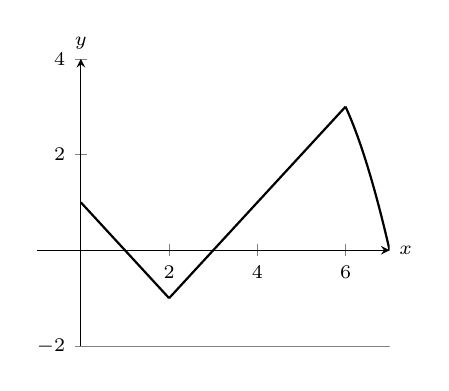
\begin{tikzpicture}
 \begin{axis}[width=.5\textwidth,tick label style={font=\scriptsize},
  axis y line=middle, axis x line=middle, name=myplot, axis on top,
  xmin=-1,xmax=7,ymin=-2,ymax=4, smooth]
  \addplot [smooth,thick,draw={\colorone},domain=0:2] {1-x};
  \addplot [smooth,thick,draw={\colorone},domain=2:6] {x-3};
  \addplot [smooth,thick,draw={\colorone},domain=6:7] {10*x-x*x-21};
  \draw [help lines,step=100] (axis cs:0,-2) grid (axis cs:7,4);
  % why steps=100?  I have no idea
 \end{axis}
 \node [right] at (myplot.right of origin) {\scriptsize $x$};
 \node [above] at (myplot.above origin) {\scriptsize $y$};
\end{tikzpicture}}{\mbox{}\\[-2\baselineskip]\begin{enumerate}
\item
\begin{tabular}{|c||c|c|c|c|c|c|c|}\hline
x & 0 & 1 & 2 & 3 & 4 & 5 & 6 \\\hline
g(x) & 0 & .5 & 0 & -.5 & 0 & 1.5 & 4 \\\hline
\end{tabular}
\item $g(7)\approx 5.7$
\item min at $x=3$; max at $x=7$
\item Approximately\\
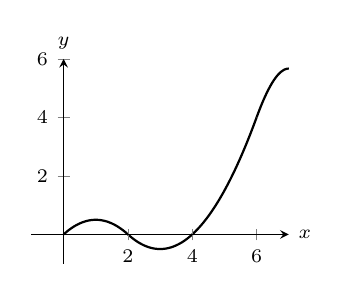
\begin{tikzpicture}
 \begin{axis}[width=.4\textwidth,tick label style={font=\scriptsize},
  axis y line=middle, axis x line=middle, name=myplot, axis on top,
  xmin=-1,xmax=7,ymin=-1,ymax=6, smooth]
  \addplot [smooth,thick,draw={\colorone},domain=0:2] {x-x*x/2};
  \addplot [smooth,thick,draw={\colorone},domain=2:6] {x*x/2-3*x+4};
  \addplot [smooth,thick,draw={\colorone},domain=6:7] {5*x*x-x*x*x/3-21*x+22};
%  \draw [help lines,step=100] (axis cs:0,-1) grid (axis cs:7,6);
 \end{axis}
 \node [right] at (myplot.right of origin) {\scriptsize $x$};
 \node [above] at (myplot.above origin) {\scriptsize $y$};
\end{tikzpicture}
\end{enumerate}}

\exercise{For any $x>0$, define
\[g(x)=\int_1^x\frac1t\ dt.\]
\begin{enumerate}
\item Show that $g(x)$ is continuous and differentiable on $(0,\infty)$ with $g'(x)=\frac1x$.
\item Show that for any positive $x$ and $y$ we have $g(xy)=g(x)+g(y)$.\\{}
[Hint: Treat $y$ as a constant, consider the derivative with respect to $x$ of each side of the proposed equation, and apply \autoref{thm:antideriv_const}.]
\item Show that for any positive $x$ and any $r$ we have $g(x^r)=rg(x)$.\\{}
[Hint: Consider the derivative with respect to $x$ of each side of the proposed equation and apply \autoref{thm:antideriv_const}.]
\end{enumerate}}{\mbox{}\\[-2\baselineskip]\begin{enumerate}
\item This is a consequence of \autoref{thm:FTC1}.
\item The derivative of the left is $g'(xy)y=\frac1{xy}y$.  The derivative of the right is $g'(x)=\frac1x$. \autoref{thm:antideriv_const} tells us that the left and right therefore differ by a constant.  Looking at $x=1$ and $g(1)=0$ tells us that this difference is 0.
\item The derivative of the left is $g'(x^r)rx^{r-1}=\frac1{x^r}rx^{r-1}$.  The derivative of the right is $rg'(x)=r\frac1x$. \autoref{thm:antideriv_const} tells us that the left and right therefore differ by a constant.  Looking at $x=1$ and $g(1)=0$ tells us that this difference is 0.
\end{enumerate}}

%\printreview

%\exerciseset{In Exercises}{, use the Fundamental Theorem of Calculus Part 1 to find $F'(x)$.
}{

\exercise{$\ds F(x) = \int_2^{x^3+x} \frac{1}{t}\ dt$
}{$F'(x) = (3x^2+1)\frac{1}{x^3+x}$
}

\exercise{$\ds F(x) = \int_{x^3}^{0} t^3\ dt$
}{$F'(x) = 3x^{11}$
}

\exercise{$\ds F(x) = \int_{x}^{x^2} (t+2)\ dt$
}{$F'(x) = 2x(x^2+2)-(x+2)$
}

\exercise{$\ds F(x) = \int_{\ln x}^{e^x} \sin t\ dt$
}{$F'(x) = e^x\sin (e^x) - 1/x\sin(\ln x)$
}
}
